

% ----------------------------------------------------------------------
% D- Módulo de estimación de la trayectoria
% - Objetivo del módulo				
% - Interfaz de los algoritmos de localización	
% - Explicación básica del procesado de medidas y estimación de la trayectoria

\subsection{Procesamiento}

En esta sección se encuentran los algoritmos capaces de generar estimaciones de la trayectoria a partir de las señales generadas. Por defecto, se encuentra implementado el filtro de Kalman extendido (EKF)\cite{Mycielski1992}. El cual da buenos resultados para simulaciones relativamente simples. De la misma forma que en las anteriores secciones los algoritmos sean parámetros de entrada del \emph{framework}, por lo que se ha diseñado para que sea fácilmente ampliable. Para ello, es necesario que los algoritmos desarrollados contengan una estructura predefinida. Este formato se muestra en la figura \ref{schemaPro}.

Los algoritmos deberán proporcionar una matriz de estimación que luego será transformada a un objeto \emph{traj}. De esta forma podemos reutilizar todos los metodos creados para las trayectorias, también para la estimaciones. 

\begin{figure}
    \centering
    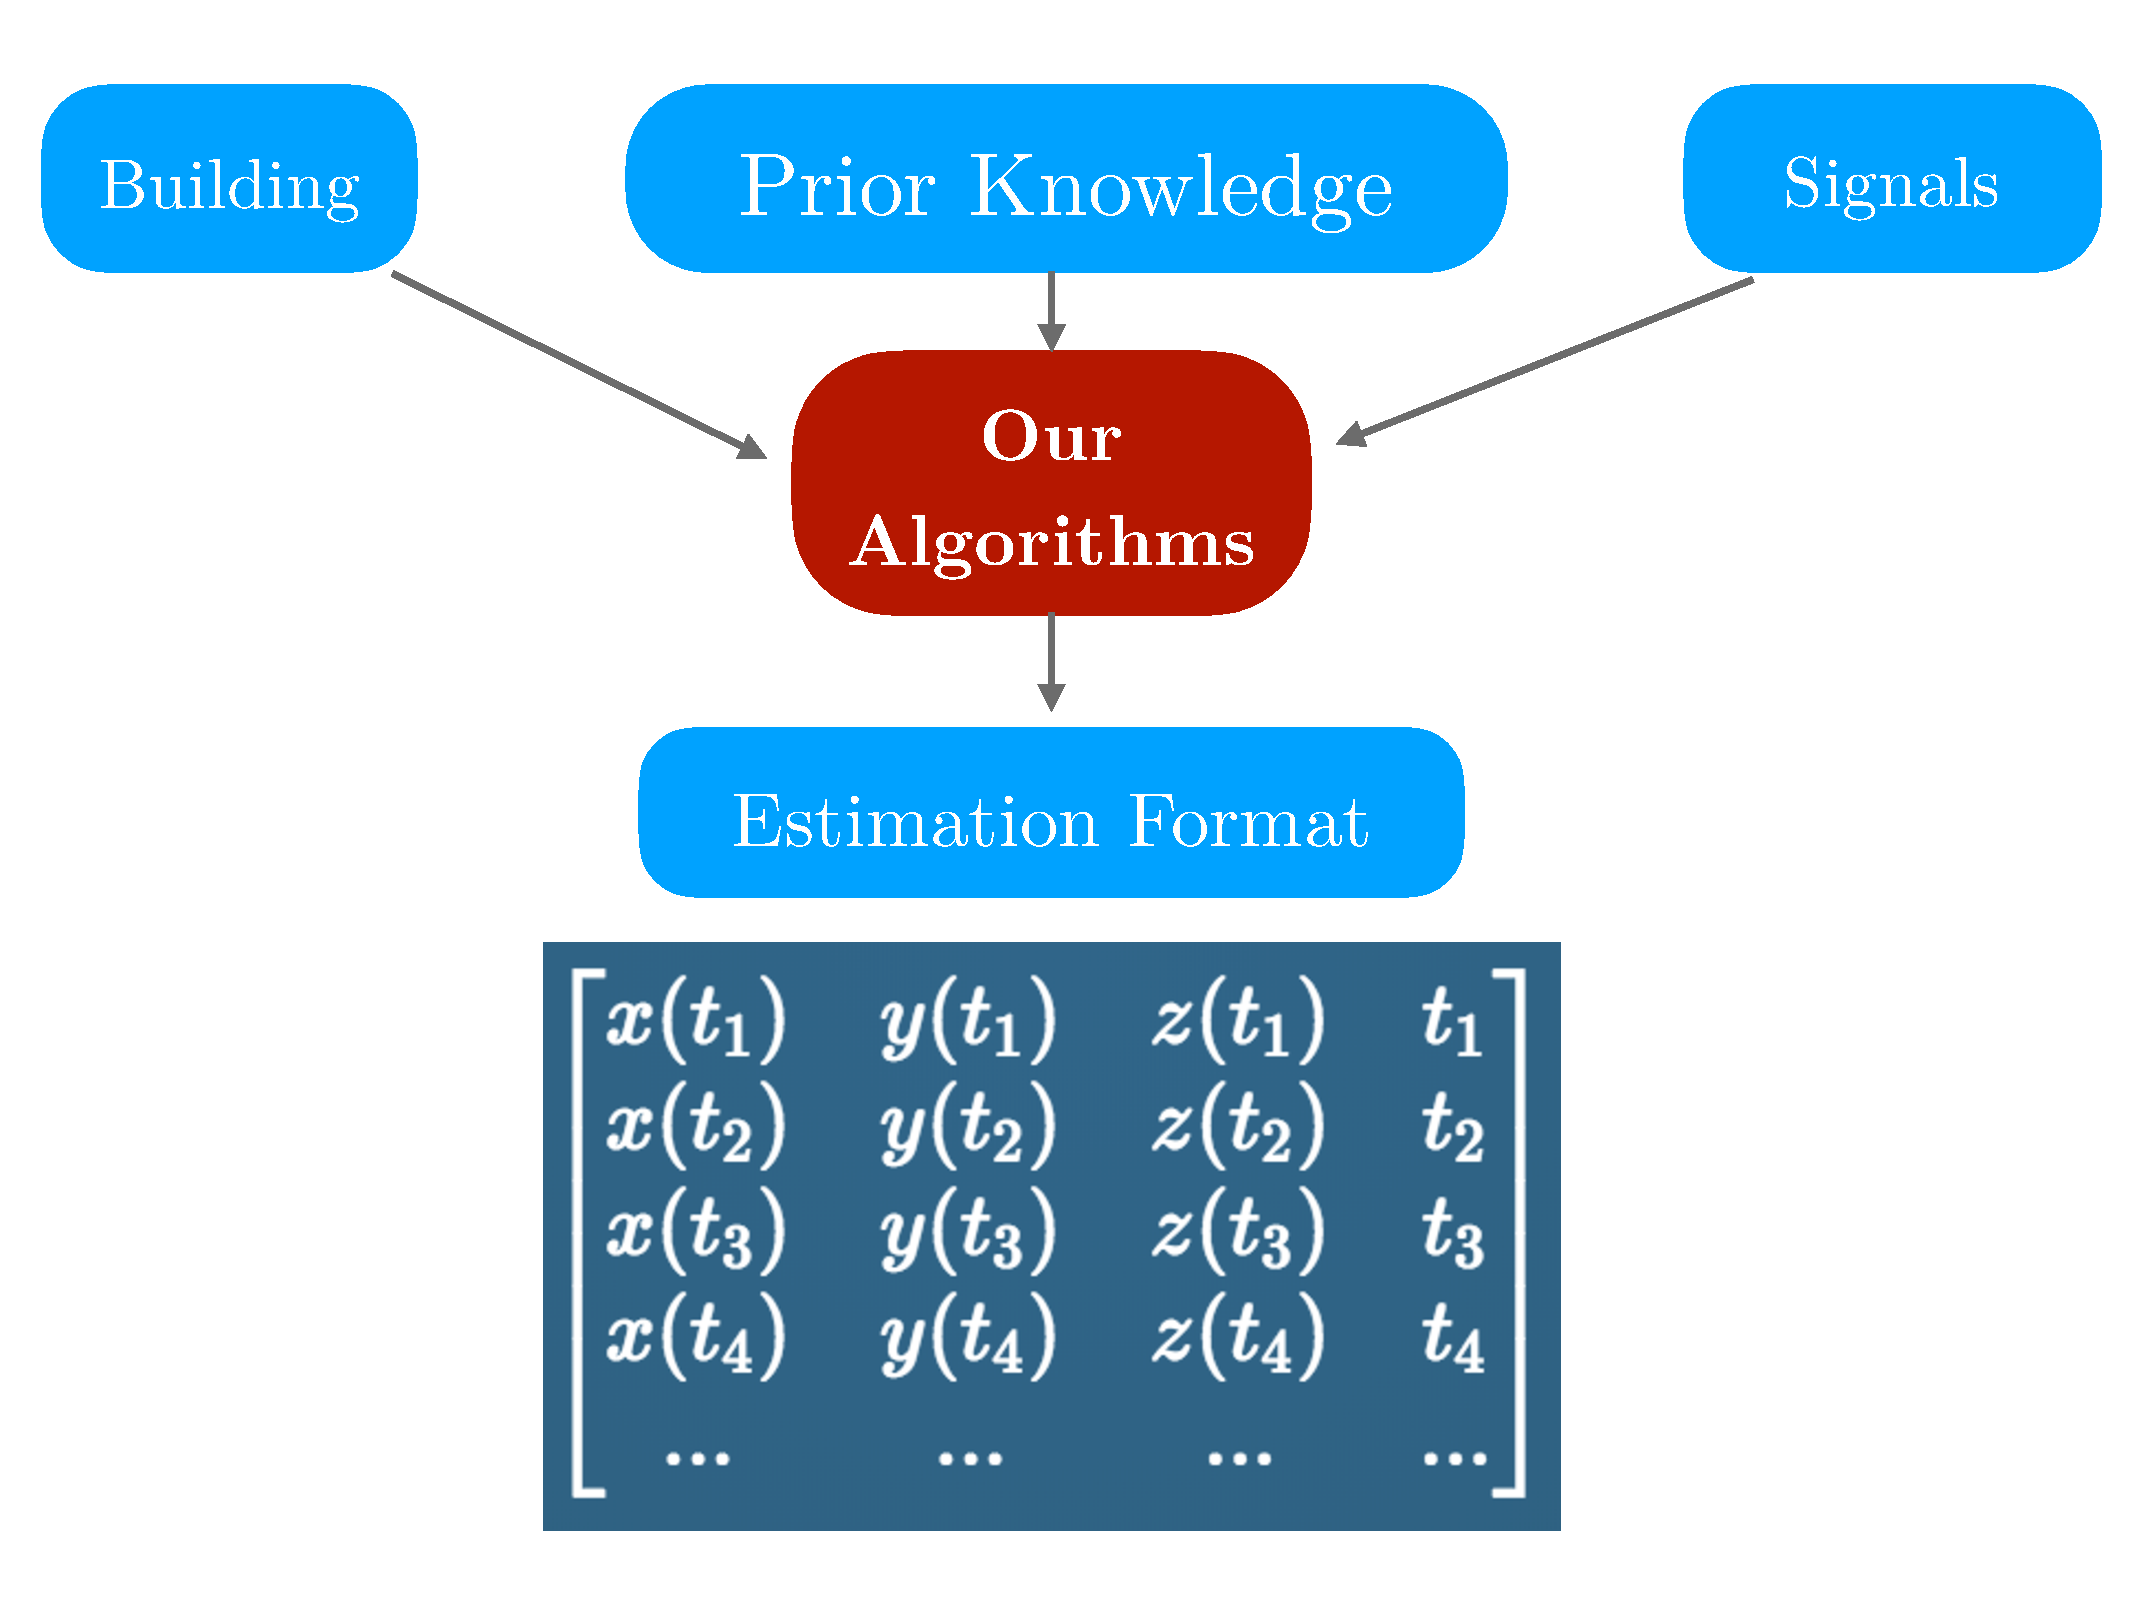
\includegraphics[width=0.8\columnwidth]{img/Design/5.pdf}
    \caption[]{Esquema del formato de entrada y de salida}
    \footnotesize 
    Los algoritmos en navindoor son funciones de MATLAB que deben tener las variables de entrada mostradas en el esquema. Los elementos como building o Signals pueden ser procesados con herramientas proporcionadas por el framework. Además tambien se puede explorar las propiedades de cada elemento para procesarlo.
    \label{schemaPro}
\end{figure}

